\section{Theory} \label{sec:theory}

\subsection{Sound analysis}
In sound analysis, one can either analyze the raw sound files directly or convert them to simpler files and hope we have not lost any essential features. A big advantage with the latter, is that the dimensionality and complexity of the data set is significantly reduced, but we will also loose some information. 

\subsubsection{Time domain}
Sounds are longitudinal waves which actually are different pressures in the air. They are usually represented as a function in the time domain, which means how the pressure vary per time. This function is obviously continuous, but since computers represent functions as arrays, we cannot save all the information. 

INSERT FIGURE

How much information we loose depends on the sampling rate, which is the number of sampling points per second. A rule of thumb is that one should have twice as high sampling rate as the highest sound frequency to keep the most important information. For instance, a human ear can perceive frequencies in the range 20-20000Hz, so around a sampling rate around 40kHz should be sufficient to keep all the information. Ordinary CD's use a sampling rate of 44.1kHz, but for speech recognition, 16kHz is enough to cover the frequency range of human speech. [https://medium.com/@ageitgey/machine-learning-is-fun-part-6-how-to-do-speech-recognition-with-deep-learning-28293c162f7a] 

\subsubsection{Frequency domain}
Sometimes, a frequency domain gives a better picture than the time domain. On one hand, one looses the time dependency, but on the other one gets information about which frequencies that are found in the wave. One goes from the time domain to the frequency domain using Fourier transformations. Which one that gives the best results in our case is not clear. 

INSERT FIGURE

\subsubsection{Extract features}
There are many techniques 

\textbf{Mel Frequency Cepstral Coefficient (MFCC)}


\textbf{Mel Spectrograms}


\subsection{Urban Sound Challenge}
\subsubsection{About the challenge}
The Urban Sound Challenge is a classification contest provided by Analytics Vidhya with the purpose of introducing curious people to a real-world classification problem. After registered, one is provided with a dataset containing sounds from ten classes. For the training data set, the classes (targets) are given, but there is also a test dataset where the targets are unknown. Our task is to classify the test dataset correctly, and by uploading our results to Analytics Vidhya's webpage, they will return the accuracy score. Participants are expected to summit their answers by 31st of December 2018, and there will be a leaderboard. We are allowed to use all possible tools, including open-source libraries like TensorFlow, Keras and Scikit-Learn. For more practical information, see [\url{https://datahack.analyticsvidhya.com/contest/practice-problem-urban-sound-classification/}]

The data sets consists of a total number of 8732 sound samples (5434 training sets and 3298 test sets) with a constant sampling rate of 22050Hz. The length of each sampling is maximum 4 seconds, and they are distributed between ten classes, namely
\begin{multicols}{2}
\begin{itemize}
	\setlength\itemsep{0.2em}
	\item air conditioner
	\item car horn
	\item children playing
	\item dog bark
	\item drilling
\end{itemize}

\columnbreak

\begin{itemize}
	\setlength\itemsep{0.2em}
	\item engine idling
	\item gun shot
	\item jackhammer
	\item siren
	\item street music
\end{itemize}
\end{multicols}

The error is evaluated with the accuracy score, which is just how much of the data set that is classified correctly:
\begin{empheq}[box={\mybluebox[5pt]}]{equation}
\text{Accuracy}=\frac{\sum_{i=1}^NI(y_i=t_i)}{N}.
\end{empheq}

\subsubsection{Examples}

ADD SOME EXAMPLES

\begin{figure} [H]
	\centering
	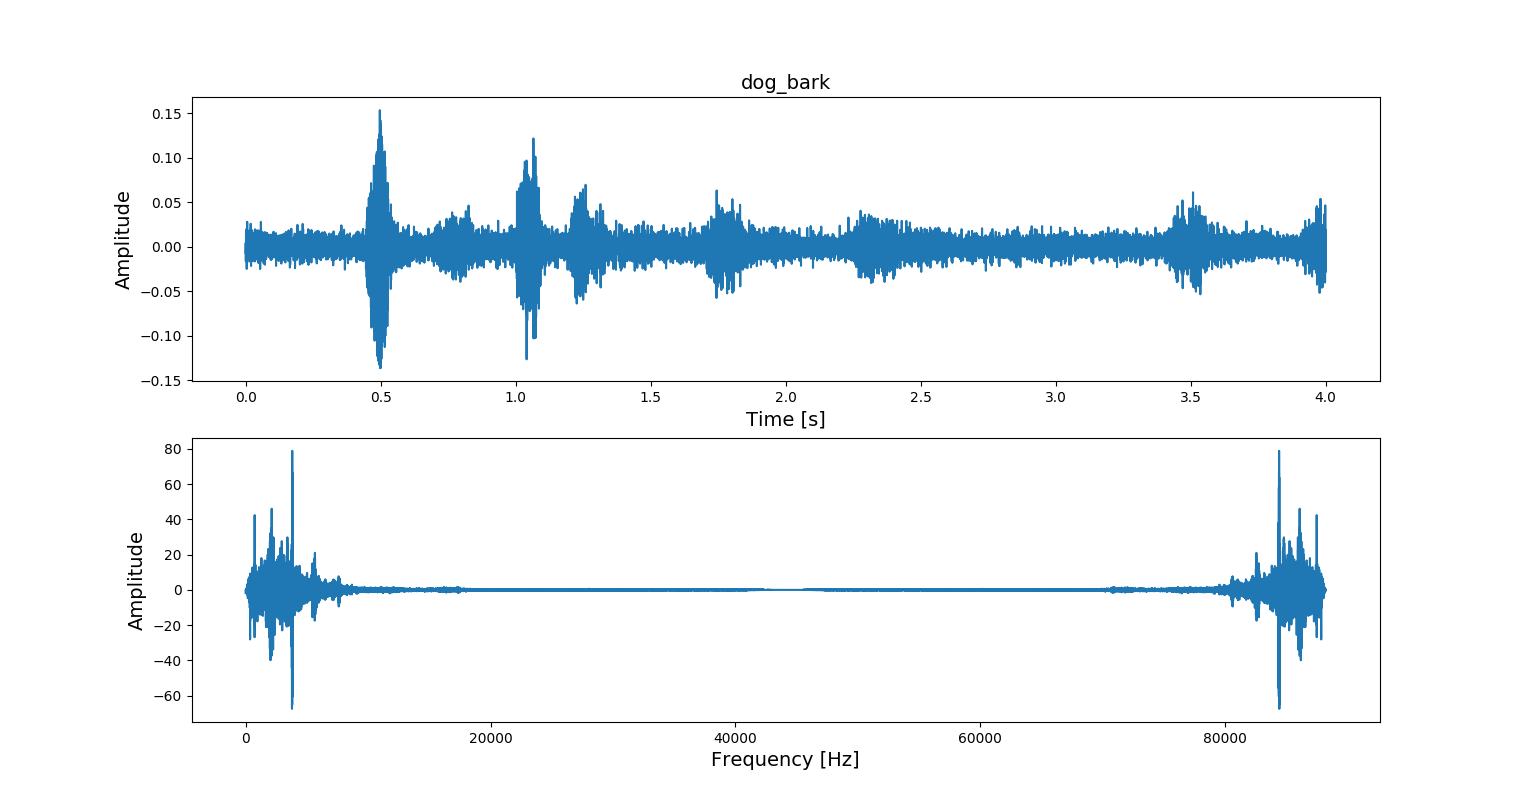
\includegraphics[scale=0.4]{../plots/dog_bark_freq.png}
	\caption{}
	\label{fig:dog}
\end{figure} 
